\documentclass[10pt, a4paper]{article}

\usepackage{hyperref}
\usepackage{listings}
\usepackage{todonotes}
\usepackage{graphicx}
\usepackage[section, below]{placeins}
\usepackage{amsmath}

\parindent 0pt

\title{Documentation of Nirs Scripts}
\author{L.Beichert(at)stud.uni-heidelberg.de}
\date{\today}


\begin{document}
\maketitle
\section*{}
This file serves as a brief documentation of the Matlab-scripts found on \url{https://github.com/lbeichert/nirs-scripts}. The purpose of these scripts is to help with the analysis of multimodal nirs and systemic data.
\section{Requirements}
The scripts work with nirs/systemic(/phosphorus) data structs as they are created by the nirs data synchronisation scripts (\url{https://github.com/aot/ucl-nirs-analysis}).
The data structs are expected to be save into files called 'pigData.m'.
The sub-folder \url{/tools} must be included in the Matlab-path in order to be able to run the other scripts.

\section{overviewPlots}
Used like:

\begin{lstlisting}
>> overviewPlots(pigDataNTB)
\end{lstlisting}

Creates an overview plot of every subject in the data-struct 'pigDataNTB' (use loadData to load) and saves it as .pdf and .fig file under \url{overviewPlots/output/}.

\begin{figure}[h]
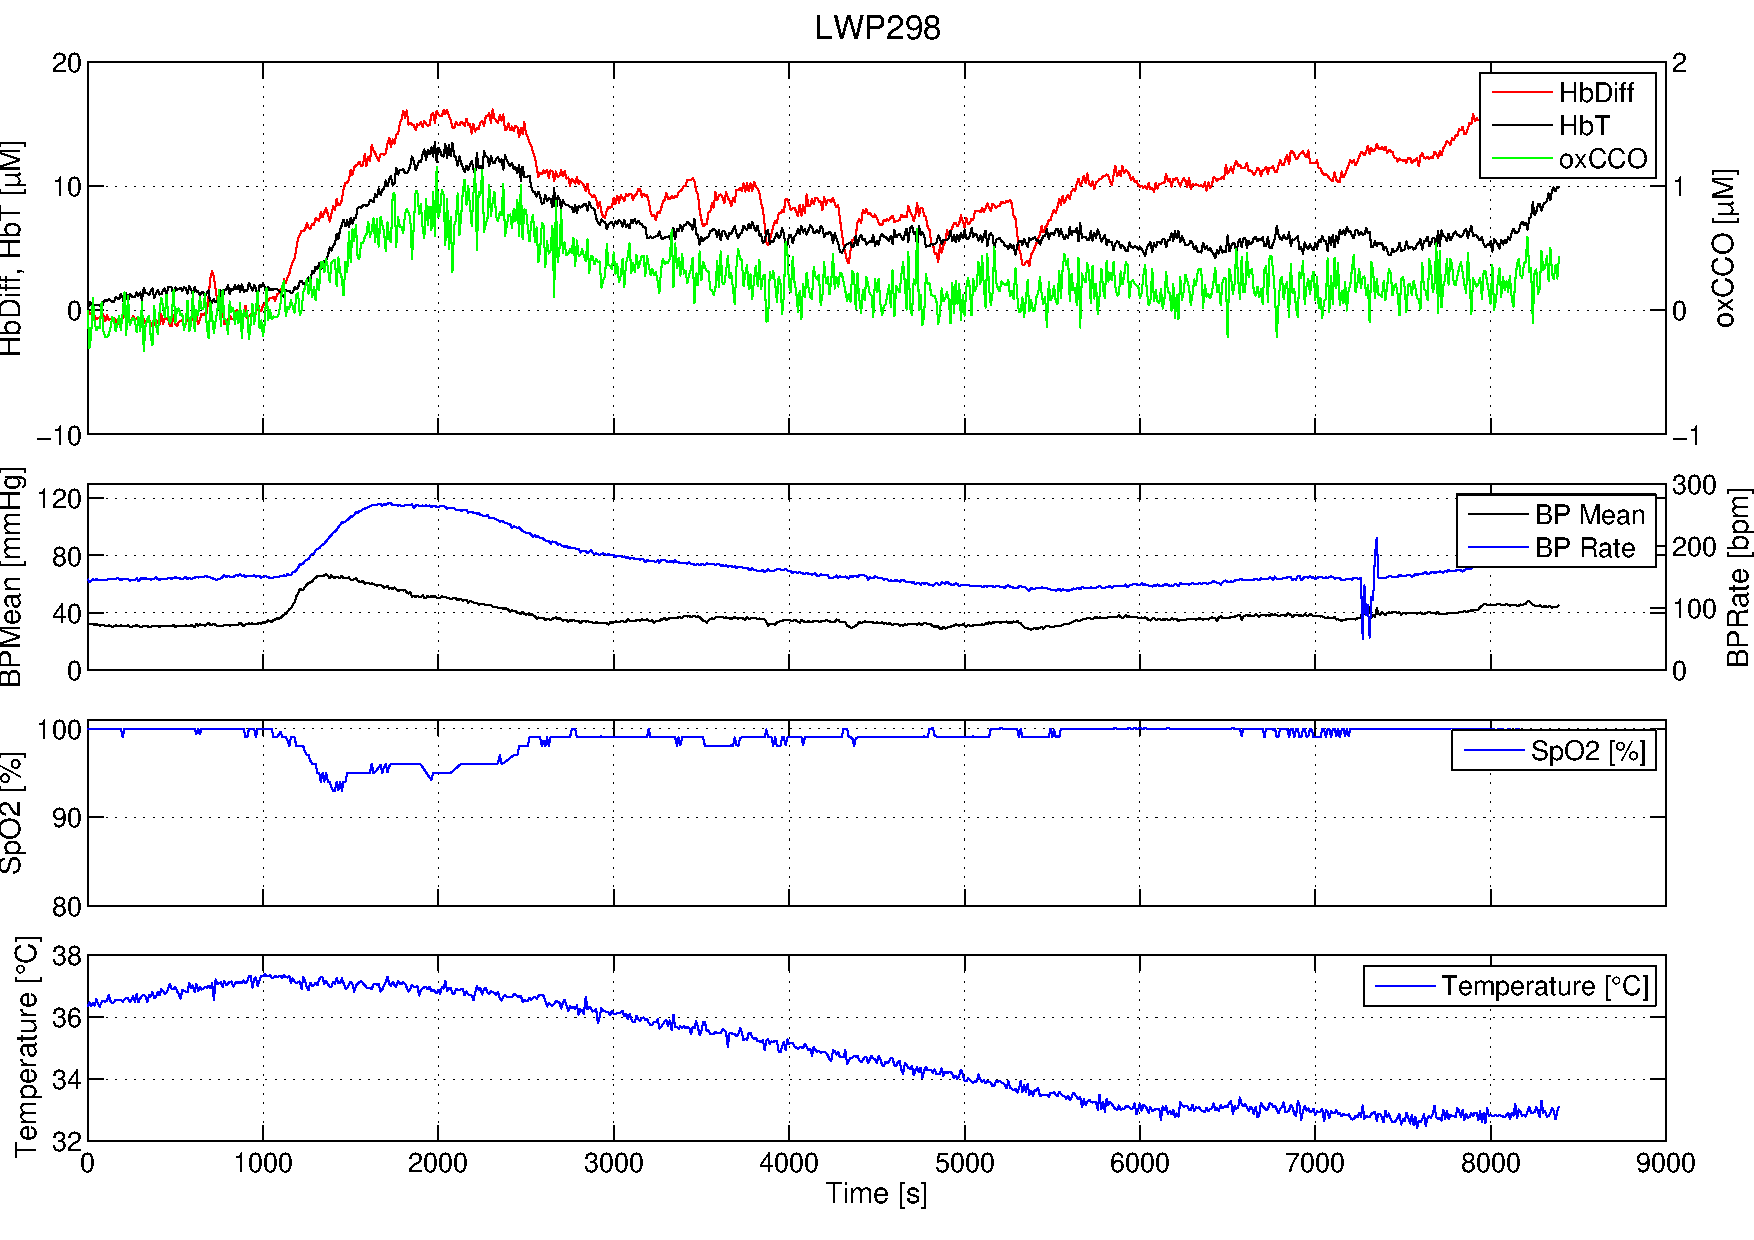
\includegraphics[width=0.9\textwidth]{LWP298_Argon_Raw.pdf}
\caption{Sample overview plot created with overviewPlots}
\end{figure}


\section{diffsBeforeAfter}
Used like:

\begin{align*}
>> results = diffsBeforeAfter(&pigData,signalName,tempStart,\\&tempTarget,plots)
\end{align*}

where signalName = 'HbDiff'/'CtOx'/... , tempStart and tempTarget something like 37.0 and 33.5, plots = (true/false) plots wanted or not.

Alternatively use:

\begin{lstlisting}
>> results = diffsBeforeAfterAll(pigData)
\end{lstlisting}

which calls diffsBeforeAfter for a number of important signals. tempStart/tempTarget are to be changed in the script.

The function takes 20 data points of a signal from around the time where temperature=tempStart and temperature=tempTarget and calculates the difference between the averages of the two sets of data points. It also performs a t-test or wilcoxon test in order to check if the calculated difference is statistically significant.
The results are saved into two excel-sheets, one with the raw numerical data and one that is more readable.

\begin{figure}[h]
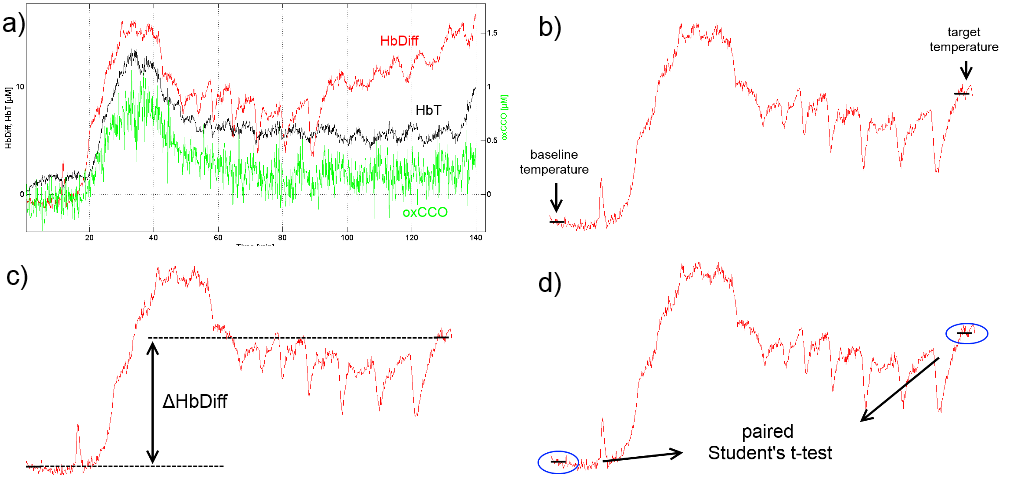
\includegraphics[width=\textwidth]{diffsBeforeAfter}
\caption{Sketch of data analysis performed by diffsBeforeAfter}
\end{figure}


\section{recoveryFraction}
Used like:
\begin{lstlisting}
>> results = recoveryFractionAll(pigData,signalName,halfWidth)
\end{lstlisting}
where signalName='HbDiff'/'CtOx'/..., halfWidth=half width of averaging window.

The script provides a graphical user interface to determine the recovery fraction. 

\paragraph {} How to use: 
\begin{itemize}
\item Start the script. A plot is displayed.
\item Click into the plot where the baseline level of the signal is supposed to be taken. A black line symbolises the selected data points and the average value.
\item If you are happy with the selection click the 'baseline' button. The average value and standard deviation is displayed on the button.
\item Repeat for insult level and recovery level.
\item Click the 'Done'-Button. A plot of the next individual appears.
\item Once you are done with all the data set, an array recoveryData is returned each of whose line consists of: ID, value and std of baseline, insult and recovery, recovery fraction
\item The recovery fraction is calculated like 
\begin{equation*}
recoveryFraction = \frac{recovery-insult}{baseline-insult} \cdot 100\%
\end{equation*}
\end{itemize}

\begin{figure}[h]
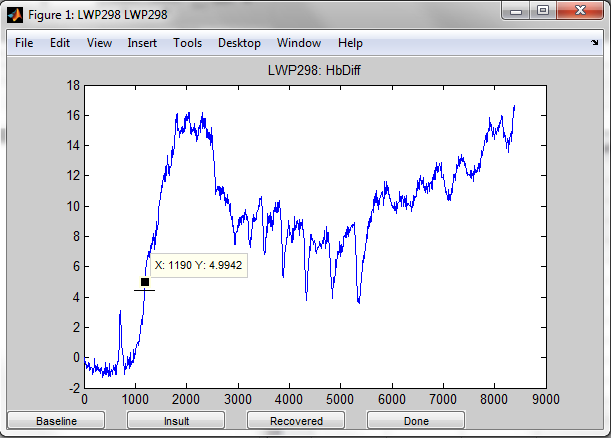
\includegraphics[width=0.9\textwidth]{recoveryFraction}
\caption{GUI of recoveryFraction (showing non-insult data)}
\end{figure}

\section{tools}
\subsection*{loadData(suffix)}
Used like:

\begin{lstlisting}
>> loadData('31p')
\end{lstlisting}

Loads pigData-structs of type 'suffix'(31p, 1h, cooling, ...) into workspace variable 'pigDataNTB'. 

Expects the structs to be saved as files called 'pigData.m' under the location \url{pigletdatadir/argon-dex/output/suffix/}. The path to the data directory must be saved as MATLAB-appdata 'pigletdatadir'. This can be done by copying the 'startup.m' file from \url{/tools} to the home directory of MATLAB and editing it according to the local path or by integrating the lines into a pre-existing startup-file. 

\subsection*{printFigure}
Used like:
\begin{lstlisting}
>> printFigure(figureHandle,path)
\end{lstlisting}
Saves figure with handle figureHandle to path in .png and landscape .pdf format.



\end{document}
